\chapter{Simple Linear Regression}

The regression model is to explain variability in independent variable by 
means of one or more of independent pr control variables.

A \textbf{simple regression model} can be expressed as
\begin{align*}
    \text{Value of dependent variable} &= 
    y\text{-intercept} + (\text{Slope} \times \text{Value of Indep. variable}) + 
    \text{Error}\\
    \mathbf{y} &= \beta_0 + \beta \mathbf{x} + \varepsilon.
\end{align*}
where $\epsilon \sim N(0, \sigma^2)$ is the error term. The sufficient statistics for the parameters $\beta_0$, $\beta_1$, and $\sigma^2$ can be derived from the likelihood function.

Now consider that we observe five pairs of $x$ and $y$ observations as follow: $(-2, 0)$, $(-1, 0)$, $(0, 1)$, $(1,1)$ and $(2, 3)$.

\begin{figure}[ht]
    \pgfplotsset{compat=1.12}
    \begin{center}
        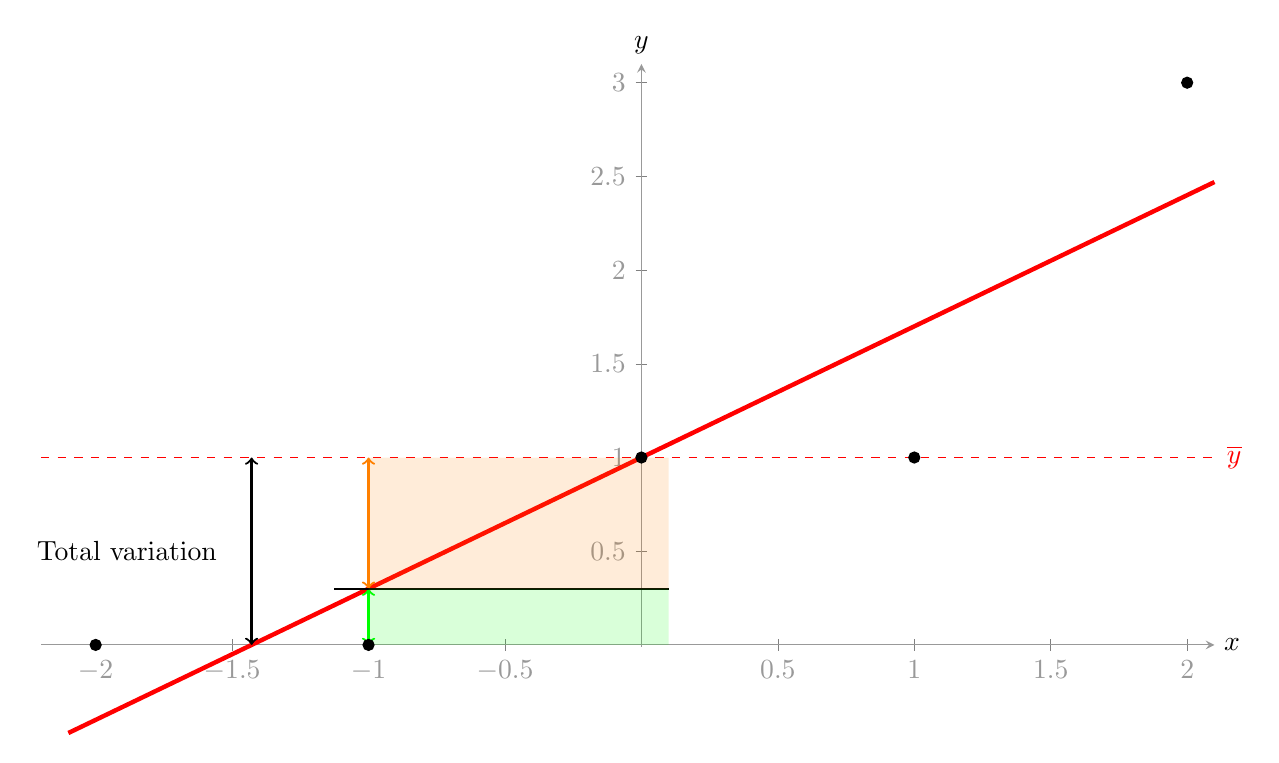
\begin{tikzpicture}
            \begin{axis}[
                scale = 1.2,
                height=7.75cm,
                width=14cm, 
                xmin=-2.2, xmax=2.1, 
                ymin=-0.01, ymax=3.1, 
                axis lines=middle,
                axis line style={gray!80!white},
                every axis label/.append style ={gray!80!white},
                every tick label/.append style={gray!80!white},
                clip=false
            ]
            \node [right] at (2.1,0) {$x$};
            \node [above] at (0, 3.1) {$y$};
            \addplot [only marks] table {
                -2 0
                -1 0
                0 1
                1 1
                2 3
            };
            \addplot[domain=-2.1:2.1, color=red, samples=200, line width=0.75pt, ultra thick]{1 + 0.7*x};
            \addplot[color = red, dashed] coordinates {(-2.2, 1) (2.1, 1)};
            \node [right, color=red] at (2.11,1) {$\overline{y}$};
            \draw[thick,<->, color=green] (-1, 0)--(-1, 0.3);
            \draw[thick,<->, color=orange] (-1, 0.3)--(-1, 1);
            \draw[thick,<->] (-1.4285, 0)--(-1.4285, 1);
            \draw[thick] (-1.125, 0.3)--(0.1, 0.3);
            \addplot[fill=orange, fill opacity=0.15, draw=none] (-1, 0.3)-- (-1, 1) -- (0.1, 1) -- (0.1, 0.3) -- cycle;
            \addplot[fill=green, fill opacity=0.15, draw=none] (-1, 0)-- (-1, 0.3) -- (0.1, 0.3) -- (0.1, 0) -- cycle;

            \node [left] at (-1.52,0.5) {Total variation};
            %\node[left,red] at (1.65,15) {$2x^5-10x+5$}; 
            %\legend{\(2x^5 - 10x +5\)};
            %\addplot[color=red, mark=*] coordinates {(-1.601,0)};
            %\addplot[color=red, mark=*] coordinates {(1.329,0)};
            %\addplot[color=red, mark=*] coordinates {(0.507,0)};
            \end{axis}
        \end{tikzpicture}
    \end{center}
    \caption{The illustrated graphs of the parameter spaces $\Theta$ and $\Theta_0$.}
\end{figure}

\section{Least squares Method}

Let $\mathcal{X} \times \mathcal{Y} = \{ (x_i, y_i) \> | \> i = 1,2 , \ldots, n \}$ be a set of data with sample size $n$. Consider 
we have a linear regression
\begin{equation}
    \uexp[x]{Y_i | x_i} = \beta_0 + \beta_1 x_i,
\end{equation}
that is a simple straight line 
\begin{equation}
    y_i = \beta_0 + \beta_1 x_i, \quad i = 1,2,\ldots,n.
\end{equation}
Take the distance of each data points to the straight line and summing up. The sum of the squares of the 
error is given by
\begin{equation}
    \mathcal{E} (\beta_0, \beta_1) = \sum_{i=1}^{n} (y_i - \beta_0 - \beta_1 x_i)^2.
\end{equation}

The least squares estimates of the fitting parameters $\beta_0$ and $\beta_1$ are said to be those values 
which minimize the sum of squares error. That is,
\begin{equation}
    \underline{\beta} = (\widehat{\beta}_0, \widehat{\beta}_1) = \argmin_{(\beta_0, \beta_1) \in \mathbb{R}^2} \mathcal{E} (\beta_0, \beta_1).
\end{equation}

\begin{example}
The article ``Relating the Cetane Number of Biodiesel
 Fuels to Their Fatty Acid Composition: A Critical Study``
 (J. of Automobile Engr., 2009: 565-583) included the 
following data on x = iodine value (g) and y = cetane
 number for a sample of 14 biofuels (see next slide).
The iodine value (x) is the amount of iodine necessary to 
saturate a sample of 100 g of oil.

\begin{table}[h!]
    \centering
    \small
    \begin{tabular}{l|cccccccccccccccc}
    \hline
    $x$ & 132.0 & 129.0 & 120.0 & 113.2 & 105.0 & 92.0 & 84.0 & 83.2 & 88.4 & 59.0 & 80.0 & 81.5 & 71.0 & 69.2\\
    \hline
    $y$ & 46.0 & 48.0 & 51.0 & 52.1 & 54.0 & 52.0 & 59.0 & 58.7 & 61.6 & 64.0 & 61.4 & 54.6 & 58.8 & 58.0\\
    \hline
    \end{tabular}
\end{table}

\begin{figure}[ht]
    \centering
    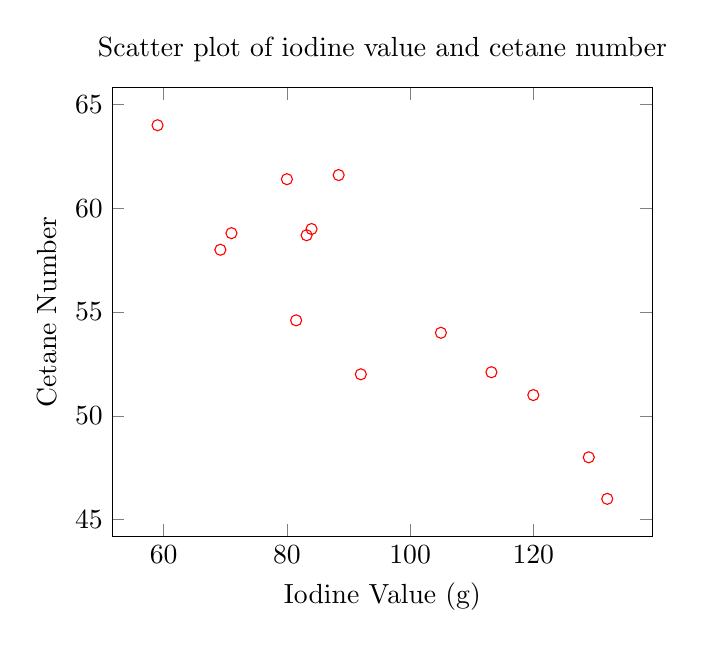
\begin{tikzpicture}
\begin{axis}[%
    title={Scatter plot of iodine value and cetane number},
    xlabel={Iodine Value (g)},
    ylabel={Cetane Number},
    scatter/classes={%
    a={mark=o,draw=red}}]
    \addplot[scatter,only marks,%
    scatter src=explicit symbolic]%
table[meta=label] {
x y label
132.0 46.0 a
129.0 48.0 a
120.0 51.0 a
113.2 52.1 a
105.0 54.0 a
92.0 52.0 a
84.0 59.0 a
83.2 58.7 a
88.4 61.6 a
59.0 64.0 a
80.0 61.4 a
81.5 54.6 a
71.0 58.8 a
69.2 58.0 a
};
\end{axis}
\end{tikzpicture}
    \caption{The scatter plot of iodine value (x) and cetane number (y).}
\end{figure}

Under the additional assumption that $\varepsilon_i$'s are iid $N(0, \sigma^2)$, the likelihood function of the sample is
\begin{align*}
    L(\alpha, \beta, \sigma^2 | \mathbf{y}, \mathbf{x}) = \prod_{i=1}^n f_Y(y_i | x_i, \alpha, \beta, \sigma^2) &= \prod_{i=1}^n \frac{1}{\sqrt{2\pi\sigma^2}} \exp\left(-\frac{(y_i - \alpha - \beta x_i)^2}{2\sigma^2}\right)\\
    &= \frac{1}{(2\pi\sigma^2)^{n/2}} \exp\left(-\frac{1}{2\sigma^2} \sum_{i=1}^n (y_i - \alpha - \beta x_i)^2\right). \label{eq:s2.1} \tag{{\color{gray} $\spadesuit $}} 
\end{align*}

Considering $(y_1, x_1), \ldots, (y_n, x_n)$ as $n$ pairs of data points plotted 
in the $xy$-plane as the scatterplot in the previous figure.

Think of drawing through this cloud of points a straight line that comes
``as close as possible`` to all the points, measured by the vertical
 distances from the points to the straight line. For any line 
$y = \alpha + \beta x$, the vertical distance from the point $(x_i, y_i)$ to the line is $y_i - (\alpha + \beta x_i)$.
Letting
\[
    \psi(\alpha, \beta) := \sum_{i=1}^n (y_i - \alpha - \beta x_i)^2,
\]

Maximizing the likelihood is equivalent to
\[
    \min_{\alpha, \beta} \sum_{i=1}^n (y_i - \alpha - \beta x_i)^2,
\]

Taking the partial derivatives of $\psi(\alpha, \beta)$ with respect to $\alpha$ and $\beta$, we have
\[
    \pdv{\psi(\alpha, \beta)}{\alpha} = -2 \sum_{i=1}^n (y_i - \alpha - \beta x_i) = 0,
\]
\[
    \pdv{\psi(\alpha, \beta)}{\beta} = -2 \sum_{i=1}^n x_i (y_i - \alpha - \beta x_i) = 0. \label{eq:s2.0} \tag{{\color{orange!50!white} $\clubsuit $}}
\]
The first equation gives
\[
    \overline{y} - a -b\overline{x} \implies a = \overline{y} - b\overline{x}.
\]
Substituting $a$ into the second equation \eqref{eq:s2.0} by $\overline{y} - b\overline{x}$ results in
\[
    \sum_{i=1}^n x_i (y_i - \overline{y}) + b \sum_{i=1}^n x_i (\overline{x} - x_i) = 0.
\]
This equation is the same as $S_{xy} = b S_{xx}$, that is
\[
    S_{xy} = \sum_{i=1}^n (x_i - \overline{x})(y_i - \overline{y}), \quad S_{xx} = \sum_{i=1}^n (x_i - \overline{x})^2.
\]
Therefore, replacing $y_i$ by the random variable $Y_i$ for all $i = 1, 2, \ldots, n$ (and we 
still use $S_{xy}$ when $y_i$ is replaced by $Y_i$), we obtain the MLE or LSE as 
\begin{equation}
    \widehat{\beta} = \frac{S_{xy}}{S_{xx}}, \quad \widehat{\alpha} = \overline{Y} - \widehat{\beta} \overline{x} = \overline{Y} - \frac{S_{xy}}{S_{xx}} \overline{x}.
\end{equation}
We can always assume that $S_{xx} > 0$, since $S_{xx} = 0$ is the trivial case of identical $x_i$'s.

We now proceed to show that $\widehat{\alpha}$ and $\widehat{\beta}$ are UMVUE of $\alpha$ and $\beta$, respectively. First of all, 
we had already shown that they are unbiased estimators of $\alpha$ and $\beta$, respectively.
\[
    \mathbb{E}[S_{xy}] = \sum^n_{i=1} (x_i - \overline{x}) \mathbb{E}_y(y_i - \overline{y}) = \sum^n_{i=1} (x_i - \overline{x}) \beta (x_i - \overline{x}) =  \beta S_{xx}.
\]
Since $\widehat{\beta}$ is unbiased for $\beta$ and 
\[
    \mathbb{E}[\widehat{\alpha}] = \mathbb{E}[\overline{Y}] - \overline{x} \mathbb{E}[\widehat{\beta}] = \alpha + \beta \overline{x} - \overline{x} \beta = \alpha.
\]
Continue with \eqref{eq:s2.1}, the likelihood function of the sample is
\begin{align*}
    L(\alpha, \beta, \sigma^2 | \mathbf{y}, \mathbf{x}) &= \frac{1}{(2\pi\sigma^2)^{n/2}} \exp\left(-\frac{1}{2\sigma^2} \sum_{i=1}^n (y_i - \alpha - \beta x_i)^2\right)\\
    &= \frac{1}{(2\pi\sigma^2)^{n/2}} \exp\left(-\frac{1}{2\sigma^2} \left[ \sum_{i=1}^n (y_i - \overline{y})^2 + n(\overline{y} - \alpha - \beta \overline{x})^2 + (\beta - \widehat{\beta})^2 S_{xx} \right] \right).
\end{align*}

where 
\[
    S_{yy} = \sum_{i=1}^n (y_i - \overline{y})^2.
\]
We still using the notation $S_{xy}$ and $S_{xx}$ when $y_i$ is replaced by $Y_i$. From the properties of the exponential family, a complete and sufficient
statistic for $\underline{\theta} = (\alpha, \beta, \sigma^2)$ is given by $(\widehat{\alpha}, \widehat{\beta}, S_{yy})$.

Since $\widehat{\alpha}$ and $\widehat{\beta}$ are both unbiased estimators and functions of the sufficient and complete 
statistic, thus they are UMVUE of $\alpha$ and $\beta$, respectively.

\end{example}
\begin{example}[(cont.)]
    \textbf{Question: What if we remove the normality assumption? } 
    $\widehat{\alpha}$ and $\widehat{\beta}$ are still least squares estimators, but they are no longer MLEs.
    A statistical property that holds for LSE is that it is the best linear unbiased estimator (BLUE) 
    in the sense that $\widehat{\alpha}$ or $\widehat{\beta}$ has the smallest variance among all linear unbiased estimators of the form 
    \begin{equation}
        \sum^n_{i=1} d_i Y_i
    \end{equation}

If the estimator of this form is unbiased for $\beta$, then 
\begin{align*}
    \beta = \mathbb{E}_y\left( \sum^n_{i=1} d_iY_i \right) &= \sum^n_{i = 1} d_i \mathbb{E}_y[Y_i]\\
    &= \sum^n_{i = 1} d_i (\alpha + \beta x_i) & \text{from the regression line, } \widehat{Y} = \alpha + \beta x\\
    &= \alpha \sum^n_{i = 1} d_i + \beta \sum^n_{i = 1} d_i x_i & \text{linearity of summation}.
\end{align*}

holds for all $\alpha$ and $\beta$, which imples that 
\[
    \sum^n_{i = 1} d_i = 0, \quad \sum^n_{i = 1} d_i x_i = 1.
\]
A geometric description  of the BLUE of $\beta$ is given in the filgure below.

% TODO: Computation of 3d graph requires longer time, this should left 
% for last part
\begin{comment}
    \begin{figure}[ht]
        \centering
        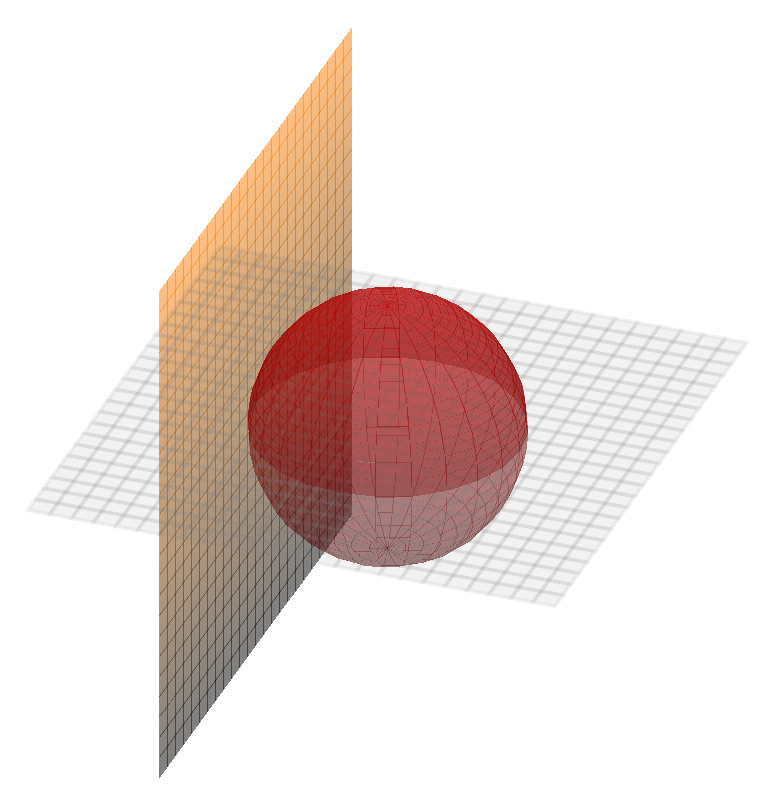
\begin{tikzpicture}[scale=3.25]
    \begin{axis}
    [   axis equal,
        hide axis,
        view={20}{30},
        z buffer=sort,
    ]
        \addplot3
        [   domain=-2:2,
            y domain=-2:2,
            surf,
            mesh/interior colormap=
           {blueblack}{color=(black) color=(orange)},
            mesh/interior colormap thresh=1,
            shader=interp,
            opacity=0.5,
        ] (-1,y,x);
        \addplot3
        [   domain=0:360,
            y domain=0:180,
            surf,
            mesh/interior colormap=
           {blueblack}{color=(black) color=(red)},
            mesh/interior colormap thresh=1,
            shader=interp,
            opacity=0.3
        ] ({sin(y)*cos(x)},{sin(y)*sin(x)},{cos(y)});
        \addplot3
        [   domain=-2:2,
            y domain=-2:2,
            surf,
            shader=flat,
            gray,
            opacity=0.1,
        ] (x,y,0);
        \addplot3
        [   domain=0:360,
            y domain=0:90,
            surf,
            mesh/interior colormap=
           {blueblack}{color=(black) color=(red)},
            mesh/interior colormap thresh=1,
            shader=interp,
            opacity=0.3,
        ] ({sin(y)*cos(x)},{sin(y)*sin(x)},{cos(y)});
    \end{axis}
\end{tikzpicture}
    \end{figure}
\end{comment}

We want to show the LSE $\widehat{\beta}$ is BLUE. Since 
\[
    Var \left( \sum^n_{i=1} d_i Y_i \right) = \sigma^2 \sum^n_{i=1} d^2_i,
\]
the BLUE of $\beta$ is the solution of the optimization problem
\begin{subequations}
\begin{alignat}{2}
&\!\min_{d_i}        &\qquad& \sum_{i=1}^{n} d^2_i\\
&\text{subject to} &      & \sum^n_{i = 1} d_i = 0,\\
&                  &      & \sum^n_{i = 1} d_i x_i = 1.
\end{alignat}
\end{subequations}

Consider the Lagrange multiplier method by minimizing 
\begin{equation}
    g(d_1, \ldots, d_n, \lambda_1, \lambda_2) = \sum_{i=1}^{n} d^2_i + \lambda_1 \left( \sum^n_{i = 1} d_i \right) + \lambda_2 \left( \sum^n_{i = 1} d_i x_i - 1 \right).
\end{equation}

Taking derivatives with respect to $d_i$ and setting them to zero, we have
\[
    \pdv{g}{d_i} = 2d_i + \lambda_1 + \lambda_2 x_i = 0.
\]
Then
\begin{align*}
    0 = \sum_{i=1}^{n} (2d_i + \lambda_1 + \lambda_2 x_i) &= 2 \sum_{i=1}^{n} d_i + n\lambda_1 + \lambda_2 \sum_{i=1}^{n} x_i & \text{linearity of summation}\\
    &= \lambda_1 n + \lambda_2 \sum^n_{i=1} x_i & \text{since } \sum d_i = 0
\end{align*}
which yields $\lambda_1 = - \lambda_2 \overline{x}$ and, hence
\[
    0 = 2d_i + \lambda_2 (x_i - \overline{x}).
\]
Then 
\[
    0 = \sum^n_{i=1} (x_i - \overline{x}) [2d_i + \lambda_2 (x - \overline{x})] = 2 + \lambda_2 S_{xx}
\]
which gives us $\lambda_2 = -2 / S_{xx}$. Then 
\[
    d_i = \frac{-(\lambda_1 + \lambda_2 x_i)}{2} = \frac{-\lambda_2(x_i - \overline{x})}{2}
    = \frac{(x_i - \overline{x})}{S_{xx}}
\]
and the BLUE of $\beta$ is 
\[
    \sum^n_{i=1} d_i Y_i = \sum_{i=1}^{n} \frac{(x_i - \overline{x})}{S_{xx}} Y_i = \frac{S_{xy}}{S_{xx}} = \widehat{\beta}.
\]
And because
\[
    \widehat{\beta} = \sum_{i=1}^{n} \frac{(x_i - \overline{x})(\beta x_i + \varepsilon_i)}{S_{xx}}
    = \beta + \sum^n_{i=1} d_i \varepsilon_i
\]
where $d_i = (x_i - \overline{x})/S_{xx}$, and the random error $\varepsilon \sim N(0,1)$. We obtain that 
\[
    Var(\widehat{\beta}) = \sum_{i=1}^{n} d^2_i Var(\varepsilon_i) = \frac{\sigma^2}{S_{xx}}.
\]
And we are done.
\end{example}

\begin{example}
    Assume monthly data of sales and advertising costs for a company below and independence between monthly sales. 
    What is the relationship between sales and advertising costs for a company?
    \begin{center}
        \begin{tabular}{c|c|c|c|c|c}
        Advertising costs (in $\$ 100,000$) & 1 & 2 & 3 & 4 & 5\\
        \hline
        Sales (in $10,000$ unit) & $1$ & $1$ & $2$ & $2$ & $4$\\
        \end{tabular}
    \end{center}
    \begin{enumerate}
        \item Find the estimated parameters $\widehat{\beta}_0$ and $\widehat{\beta}_1$. What do these estimated parameters mean?
        \item What are the estimated sales when the advertising cost is $\$ 100,000$ and $\$ 250,000$, respectively?
    \end{enumerate}
\end{example}
\begin{solution}
    \begin{enumerate}
        \item Using LSE to find unbiased estimators of the parameters:

    \begin{center}
        \begin{tabular}{c|c|c|c|c|c}
        & $x$ & $y$ & $x^2$ & $y^2$ & $xy$\\
        \hline
        & $1$ & $1$ & $1$ & $1$ & $1$\\
        & $2$ & $1$ & $4$ & $1$ & $2$\\
        & $3$ & $2$ & $9$ & $4$ & $6$\\
        & $4$ & $2$ & $16$ & $4$ & $8$\\
        & $5$ & $4$ & $25$ & $16$ & $20$\\
        \hline
        $\sum=$ & $15$ & $10$ & $55$ & $26$ & $37$\\
        \hline
        \end{tabular}
    \end{center}
    Now we can applying the formulas,
    \[
        \widehat{\beta}_1 = \frac{n\sum xy - (\sum x)(\sum y)}{n\sum x^2 - (\sum x)^2}
        = \frac{5(37) - 15(10)}{5(55)-15^2} = 0.70.
    \]
    and 
    \[
        \widehat{\beta}_0 = \ols{Y} - \widehat{\beta}_1 \ols{X} = 
        \frac{\sum y}{n} - \widehat{\beta}_0 \left(\frac{\sum x}{n} \right)
        = \frac{10}{5} - 0.70 \times \frac{15}{5} 
        = -0.10.
    \]
    The fitted regression line is $\widehat{y} = -0.1 + 0.7x$. We take a look on each estimated parameters:
    \begin{itemize}
        \item[$\bullet$] $\widehat{\beta}_0 = -0.1$, since there is no advertising cost, the sales is $-1000$ units, which is meaningless.
        \item[$\bullet$] $\widehat{\beta}_1 = 0.7$, as the advertising cost increased by $\$100,000$, the sales is increased by $7000$ units.
    \end{itemize}

    \begin{figure}[ht]
    \centering
    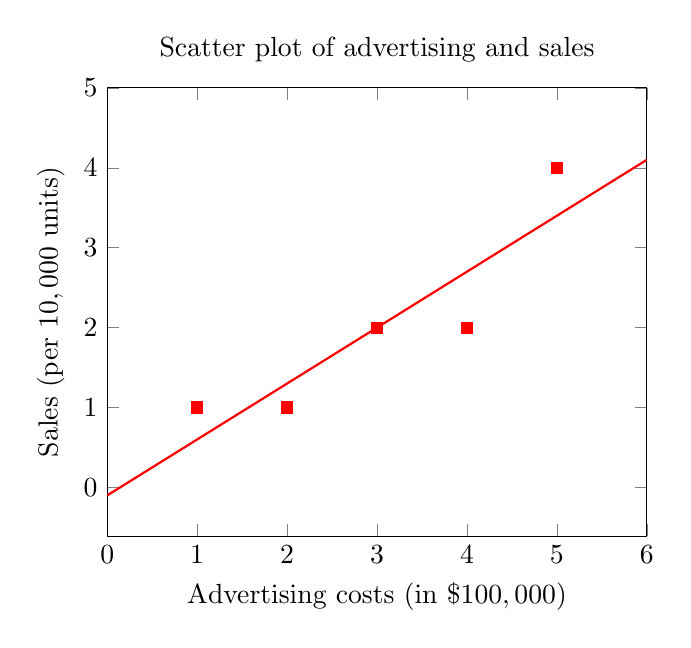
\begin{tikzpicture}
    \begin{axis}[%
        title={Scatter plot of advertising and sales},
        xmin=0, xmax=6,
        xmin=0, ymax=5,
        domain=0:6,
        xlabel={Advertising costs (in $\$ 100,000$)},
        ylabel={Sales (per $10,000$ units)},
        scatter/classes={%
        a={mark=square*,draw=red,fill=red}}]
        \addplot[scatter,only marks,%
        scatter src=explicit symbolic]%
    table[meta=label] {
    x y label
    1 1 a
    2 1 a
    3 2 a
    4 2 a
    5 4 a
    };
    \addplot[thick, red]{-0.1 + 0.7*x};
    \end{axis}
    \end{tikzpicture}
        \caption{The scatter plot of advertising costs ($x$) and sales ($y$). The scatterplot shows a positive linear relationship.}
    \end{figure}

    \item If advertising cost is $\$100,000$, that means $x=1$. The estimated sales will be $\widehat{y}_{1} = -0.1 + 0.7(1) = 0.6$. Which is 6,000 units.

    If advertising cost is $\$250,000$, that means $x=2.5$. The estimated sales will be $\widehat{y}_{2.5} = -0.1 + 0.7(2.5) = 1.65$. Which is 16,500 units.
    \end{enumerate}
\end{solution}

\begin{definition}[Extrapolation]
    \textbf{Extrapolation} is using the regression line to predict the value of a response corresponding to a $x$ values 
    that is \textbf{outside the range} of the data used to determine the regression line.

    Extrapolation may lead to \textbf{unreliable predictions}.
\end{definition}

\section{Making Inference}

\begin{lemma}
    Given the simple linear regression $Y_i = \beta_0 + \beta_1 x_i$, and each 
    $x_i$ to be a set of arbitrary but fixed real numbers, then 
    \begin{enumerate}
        \item $\CS{E} = \CS{T} - \widehat{\beta}_1 S_{xY}$.
        \item $\cov({X,Y}) = S_{xx} \widehat{\beta}_1$.
        \item $\displaystyle \cov({\widehat{\beta}_0, \widehat{\beta}_1}) = -\frac{\overline{x} \sigma^2}{S_{xx}}$.
    \end{enumerate}
\end{lemma}
\begin{proof}
    \begin{enumerate}
        \item \begin{align*}
            \CS{T} = \CS{E} + \CS{R} &\implies \CS{E} = \CS{T} - \CS{R}\\
            &\implies \CS{E} = \CS{T} - \CS{R}
        \end{align*}
    \end{enumerate}
\end{proof}

\subsection{Estimate $\sigma^2$}

The error sum of squares (equivalently, \textit{residual sum of squares}), denoted by $\CS{E}$, is 
\begin{equation}
    \CS{E} = \sum_{i=1}^{n} (y_i - \widehat{y}_i)^2 = \sum_{i=1}^n \left[y_i - (\widehat{\beta}_0 + \widehat{\beta}_1 x_i ) \right]^2
\end{equation}

and the estimate of $\sigma^2$ is 
\begin{equation}
    \widehat{\sigma}^2 = s^2 = \frac{\CS{E}}{n-2} = \frac{1}{n-2} \sum_{i=1}^n \left(y - \widehat{y}_i \right)^2
    = \frac{1}{n-2} \sum_{i=1}^{n} \widehat{\epsilon}_i^2.
\end{equation}

The divisor $n - 2$ in $S^2$ is the number of degrees of freedom associated with $\CS{E}$ and the estimate 
$s^2$. This is because to obtain the sample variance $s^2$, the two parameters $\beta_0$ and $\beta_1$ must 
first be estimated, which results in a loss of $2$ degree of freedom, just as $\mu$ had to 
be estimated in one sample problems, resulting in an estimated variance based on $n-1$ 
degree of freedom in our previous $t$-tests assumption. Indeed, $S^2$ is an unbiased estimator for $\sigma^2$.

\begin{theorem}[Unbiased Estimator for $\sigma^2$]
    Given the simple linear regression $Y_i = \beta_0 + \beta_1 x_i$, then 
    \begin{equation}
        \MS{E} = S^2 = \frac{1}{n-2} \CS{E} = \frac{1}{n-2} \sum_{i=1}^{n} \left(Y_i - \widehat{Y}_i\right)^2
    \end{equation}
    is an unbiased estimator for population variance $\sigma^2$.
\end{theorem}
\begin{proof}
    To show that $S^2$ is an unbiased estimator for $\sigma^2$, we want verify that
    \[
        \mathbb{E}[S^2] = \mathbb{E} \left[ \frac{\CS{E}}{n-2}\right]
        = \frac{1}{n-2} \mathbb{E}[\CS{E}] \stackrel{?}{=} \sigma^2,
    \]
    it is important to find $\mathbb{E}[\CS{E}]$ in order to verify the identity above.

    Notice that
    \begin{align*}
        \mathbb{E}[\CS{E}] &= \mathbb{E} \left[ \sum_{i=1}^{n} \left(Y_i - \widehat{Y}_i\right)^2 \right]\\
        &= \mathbb{E} \left[ \sum_{i=1}^{n} (Y_i - \ols{Y} + \widehat{\beta}_1 \overline{x} - \widehat{\beta}_1 x_i)^2  \right]\\
        &= \mathbb{E} \left[ \sum_{i=1}^{n} \left((Y_i - \ols{Y}) + \widehat{\beta}_1 (\overline{x} - x_i) \right)^2  \right]\\
    \end{align*}
    continue to expand the squares and we have 
    \[
        \mathbb{E}[\CS{E}]
        = \mathbb{E} \left[ \sum (Y_i - \ols{Y})^2 + \widehat{\beta}_1^2 \sum (x_i - \overline{x})^2 - 2\widehat{\beta}_1 \sum (x_i - \overline{x})(Y_i - \ols{Y}) \right]. 
        \label{eq:reg1.0} \tag{{\color{cyan} $\clubsuit$}}
    \]
    Since $\sum (x_i - \overline{x})(Y_i - \ols{Y}) = \widehat{\beta}_1 S_{xx}$, and also $\sum (Y_i - \ols{Y})^2 = \sum Y_i^2 - n\ols{Y}$. Combining these two 
    results and replace the first and last term of \eqref{eq:reg1.0}. We have 
    \begin{align*}
        \mathbb{E}[\CS{E}] &= \mathbb{E} \left[ \sum Y_i^2 - n\ols{Y} + \widehat{\beta}^2_1 S_{xx} - 2 \widehat{\beta}_1 \left(\widehat{\beta}_1 S_{xx}\right) \right]\\
        &= \mathbb{E} \left[ \sum Y_i^2 - n\ols{Y} - \widehat{\beta}^2_1 S_{xx} \right]\\
        &= \sum \mathbb{E}[Y_i^2] - n \mathbb{E} [\ols{Y}^2] - S_{xx} \, \mathbb{E}[\widehat{\beta}^2_1]. \label{eq:reg1.1} \tag{{\color{red} $\heartsuit $}}
    \end{align*}
    Applying the theorem that for any random variable $U$, $\mathbb{E}[U^2] = Var[U] - \mathbb{E}[U]^2$. We can see that 
    \begin{align*}
        \eqref{eq:reg1.1} = \mathbb{E}[\CS{E}] &= \sum^n_{i=1} \left[ V(Y_i) - \mathbb{E}[Y_i]^2 \right] - n \mathbb{E} [V(\ols{Y}) - \mathbb{E}[\ols{Y}]^2] \\
        &\quad - S_{xx} \left( \frac{\sigma^2}{S_{xx}} + \beta^2_1 \right)\\
        &= n\sigma^2 + \sum^n_{i=1} \left(\beta_0 + \beta_1 x_i \right)^2 - n \left[ \frac{\sigma^2}{n} + \left(\beta_0 + \beta_1 x_i \right)^2 \right]\\
        &\quad - S_{xx} \left( \frac{\sigma^2}{S_{xx}} + \beta^2_1 \right)\\
        &= n\sigma^2 + n\left(\beta_0 + \beta_1 x_i \right)^2 - \sigma^2 - n\left(\beta_0 + \beta_1 x_i \right)^2 - \sigma^2 - S_{xx}\beta_1\\
        &= \sigma^2(n-2).
    \end{align*}
\end{proof}

\subsection{Inference about the Slope parameter $\beta_1$}

\begin{lemma}
    In normal regression, the distributions of the slope parameters 
    $\widehat{\beta}_1$ and $\widehat{\beta}_0$ are given by
    \begin{equation}
        \widehat{\beta}_1 \sim N \left(\beta_1, \frac{\sigma^2}{S_{xx}}\right) \quad \text{ and } \quad 
        \widehat{\beta}_0 \sim N \left(\beta_0, \frac{\sigma^2}{n} + \frac{\overline{x}^2 \sigma^2}{S_{xx}}\right).
    \end{equation}
\end{lemma}
\begin{proof}
    On the other hand, now we need to determine the distribution of intercept 
    $\widehat{\beta}_0$. Since $Y_i \sim N(\beta_0 + \beta_1 x_i, \sigma^2)$, the distribution of 
    $\ols{Y}$ is given by 
    \[
        \ols{Y} \sim N \left(\beta_0 + \beta_1 \ols{x}, \frac{\sigma^2}{n} \right).
    \]
    We proved that 
    \[
        \widehat{\beta}_1 \sim N\left(\beta_1, \frac{\sigma^2}{S_{xx}} \right).
    \]
    Multiply it by $\overline{x}$ and the distribution of $\overline{x}\widehat{\beta}_1$ is given by 
    \[
        \overline{x}\widehat{\beta}_1 \sim N\left(\overline{x}\beta_1,\> \overline{x}^2 \frac{\sigma^2}{S_{xx}} \right).
    \]
    Notice that $\widehat{\beta}_0 = \ols{Y} - \overline{x}\widehat{\beta}_1$, and $\ols{Y}$ and 
    $\overline{x}\widehat{\beta}_1$ both are normal random variables. $\widehat{\beta}_0$ is also 
    normal with mean equal to $\beta_0 + \beta_1 \overline{x} - \beta_1 \overline{x} = \beta_0$ and variance 
    is equal to 
    \[
        Var[\widehat{\beta}_0] = \frac{\sigma^2}{n} + \frac{\overline{x}^2 \sigma^2}{S_{xx}}.
    \]
    That is, 
    \[
        \widehat{\beta}_0 \sim N \left(\beta_0, \frac{\sigma^2}{n} + \frac{\overline{x}^2 \sigma^2}{S_{xx}}\right)
    \]
    provided the distribution of $Y_i | x_i$ is normal. The proof of the theorem is now complete.
\end{proof}

\begin{theorem}
    The test statistic to test the hypotheses
    \[
        H_0: \beta_1 = \beta_1^* \quad \text{ against } \quad H_0: \beta_1 \neq \beta_1^*
    \]
    is 
    \begin{equation}
        T = \frac{\widehat{\beta}_1 - \beta_1^*}{S/ \sqrt{S_{xx}}} = 
        \frac{\widehat{\beta}_1 - \beta_1^*}{\widehat{\sigma}} \sqrt{\frac{(n-2) S_{xx}}{n}},
    \end{equation}
    which has a $t$-distribution with $n-2$ degree of freedom. Reject $H_0$ if 
    \[
        |T| < t_{n-2, \> \frac{\alpha}{2}}.
    \]
\end{theorem}

The term $\displaystyle Se(\widehat{\beta}_1) = \sqrt{\frac{\MS{E}}{S_{xx}}}$ is the 
estimated standard error of $\widehat{\beta}_1$. The $p$-value based on $n-2$ df can be computed as was done previously for $t$-tests.

\begin{example}
    The frequency of chirping of a cricket is thought to be related to temperature. This study 
    suggests the possibility that the temperature can be estimated through the chirp frequency. The 
    following data shown the number of chirping per second, $x$ by the striped ground cricket and the 
    temperature, $y$ in Fahrenheit:

    \begin{center}
        \begin{tabular}{c|cccccccccc}
            $x$ & 20 & 16 & 20 & 18 & 17 & 16 & 15 & 17 & 15 & 16\\
            \hline
            $y$ & 89 & 72 & 93 & 84 & 81 & 75 & 70 & 82 & 69 & 83\\
            \end{tabular}
    \end{center}
    Assuming the regression of temperature on the number of chirps per second is normal random variable. Test the 
    hypotheses
    \[
        H_0 : \beta_1 = 4 \quad \text{ against } \quad H_1 : \beta_1 \neq 4
    \]
    at the significance level $0.1$.
\end{example}

\section{Prediction}

\subsection{Prediction vs Estimation}

What is the main reason we fitting a model to data? It is often to accomplish one of two goals. We can either
use a model to estimate the relationship between response and the predictors, or to predict the response
based on the predictors. Often, a good model can do both, but here we'll discuss both goals separately since
the process of finding models for explaining and predicting are slightly different. In most cases, prediction
is less precise than estimation with a bigger standard error.

Rather than calculate an interval estimate for $\mu_{Y, x^*}$, an
investigator may wish to obtain a range or an interval of
possible values of $Y$ associated with some future
observation when the independent variable has value $x^*$. Consider, for example, relating vocabulary size $y$ to age of
a child $x$. The CI with $x^* = 6$ would provide a range that
covers with 95\% confidence the true average vocabulary
size for all 6-year-old children.

Alternatively, we might wish an interval of plausible values
for the vocabulary size of a particular 6-year-old child. How
can you tell that a child is ``off the chart'' for example?

A \textbf{confidence interval} refers to a \textit{parameter}, or population
characteristic, whose value is \textit{fixed but unknown} to us.

In contrast, a \textbf{future value} of $Y$ is not a parameter but
instead a \textit{random variable}; for this reason we refer to an
\textit{interval of plausible values for a future $Y$} as a \textbf{prediction
interval} rather than a confidence interval. Determining a prediction interval for $Y$ requires that we
model the error involved in the prediction of the $Y$ variable.

One important application in linear regression is the prediction of a future value 
$Y_0$ at the covariate value $x_0$,
\[
    Y_0 = \beta_0 + \beta x_0 + \varepsilon_0
\]
Since the mean of $Y_0$ is $\beta_0 + \beta x_0$, the commonly used predict value for $Y$ is 
\[
    \widehat{Y}_0 = \widehat{\beta_0} + \widehat{\beta} x_0
\]
which has mean $\beta_0 + \beta x_0$ and variance
\begin{align*}
    Var(\widehat{Y}_0) &= Var(\widehat{\beta_0}) + x^2_0 Var(\widehat{\beta}) + 2x_0 \cov({\widehat{\beta_0}, \widehat{\beta}}) + Var(\varepsilon_0)\\
    &= \frac{\sigma^2}{S_{xx}} \left(\frac{1}{n} S_{xx} + \overline{x}^2 + x_0^2 - 2x_0 \overline{x} \right)\\
    &= \sigma^2 \left[\frac{1}{n} + \frac{(x_0 - \overline{x})^2}{S_{xx}}\right].
\end{align*}
The prediction error $Y_0 - \widehat{Y}_0$ must have zero mean, which means it is an unbiased prediction 
and with variance 
\begin{equation}
    \sigma^2 + Var(\widehat{Y}_0) = \sigma^2 \left[1 + \frac{1}{n} + \frac{(x_0 - \overline{x})^2}{S_{xx}}\right].
\end{equation}
We would like to construct an interval $C$ based on samples data such that 
\[
    \mathbb{P}[Y_0 \in C] = 1 - \alpha
\]
This is called a prediction interval, where $\mathbb{P}$ is the probability measure 
with respect to both $Y_0$ and $Y_1, \ldots, Y_n$, then we can apply the fact that, under the 
normality assumption on $\varepsilon$'s, 
\begin{equation}
    \frac{Y_0 - \widehat{Y}_0}{\widehat{\sigma} \sqrt{1 + \frac{1}{n} + \frac{(x_0 - \overline{x})^2}{S_{xx} }} } \sim t_{\nu = n-2}
\end{equation}
The resulting interval is $C = [\widehat{Y}_-, \widehat{Y}_+]$, where
\begin{equation}
    \widehat{Y}_\pm = \widehat{Y}_0 \pm t_{n-2, \> \alpha/2}\, \widehat{\sigma} \sqrt{1 + \frac{1}{n} + \frac{(x_0 - \overline{x})^2}{S_{xx} }}
\end{equation}

\begin{theorem}[Prediction interval for Future value $Y$]
    The prediction interval of $Y$ is
    \begin{equation}
        \widehat{Y}_\pm = \widehat{Y}_0 \pm t_{n-2, \> \alpha/2}\, \widehat{\sigma} \sqrt{1 + \frac{1}{n} + \frac{(x_0 - \overline{x})^2}{S_{xx} }}
    \end{equation}
\end{theorem}

Suppose that we want to construct a confidence interval for
$\theta = \alpha + \beta x_0$, the mean of $Y$-values at $x_0$, instead of a prediction
interval for the future value $Y_0$.

We can use $\widehat{Y}_0 = \widehat{\alpha} + \widehat{\beta} x_0$ as an estimator of $\theta$ and we still have
\[
    Var(\widehat{Y}_0) = \sigma^2 \left(\frac{1}{n} + \frac{(x_0 - \overline{x})^2}{S_{xx}}\right)
\]
Under the normality assumption on $\varepsilon$'s,
\[
    \frac{\widehat{Y}_0 - \theta}{\widehat{\sigma} \sqrt{\frac{1}{n} + \frac{(x_0 - \overline{x})^2}{S_{xx}}}} \sim t\text{-distribution with degrees of freedom } n-2
\]
Hence, the resulting confidence interval is $C_0 = [\widehat{\theta}_-, \widehat{\theta}_+]$, where
\[
    \widehat{\theta}_\pm = \widehat{Y}_0 \pm t_{n-2, \> \alpha/2}\, \widehat{\sigma} \sqrt{\frac{1}{n} + \frac{(x_0 - \overline{x})^2}{S_{xx}}}
\]
This interval is \textbf{shorter} than the prediction interval for a future $Y_0$,
because of the additional variability from $Y_0$ in the prediction interval.
Without the normality assumption, $C_0$ is still asymptotically valid but $C$
is not asymptotically valid.

The interpretation of the prediction level $100(1-\alpha)\%$ is
similar to that of previous confidence levels---if is used
repeatedly, in the long run the resulting interval will actually
contain \textbf{the observed $y$ values} $100(1-\alpha)\%$ of the time.

Notice that the 1 underneath the initial square root symbol
makes the PI wider than the CI, though the intervals are
both centered at $\widehat{\beta}_0 + \widehat{\beta}_1 x^*$.

Also, as $n \to \infty$, the width of the CI approaches 0, whereas
the width of the PI does not (because even with perfect
knowledge of $\beta_0$ and $\beta_1$, there will still be randomness in
prediction).

\section{Correlation: How strong is the linear relationship?}

In regression analysis, the linear correlation coefficient (which also called \textbf{Pearson correlation coefficient}), $\rho$, 
is the measure of the degree of association between the response $x$ and explanatory data $y$.

Recall that if $X$ and $Y$ are bivariate random variables with means
$\mu_X$ and $\mu_Y$ and standard deviations $\sigma_X$ and $\sigma_Y$, respectively.

\[
    f(x,y) = \frac{1}{2\pi \sigma_1 \sigma_2 \sqrt{1 - \rho^2}} \exp \left\{ -\frac{1}{2(1 - \rho^2)} 
    \left[ \left(\frac{y - \mu_1}{\sigma_1}\right)^2 + \left(\frac{x - \mu_2}{\sigma_2}\right)^2 -2\rho \left(\frac{y - \mu_1}{\sigma_1}\right)\left(\frac{x - \mu_2}{\sigma_2}\right) \right]\right\}
\]

then the correlation coefficient between $X$ and $Y$ is defined as
\begin{equation}
    \rho_{X,Y} = \frac{\text{Cov}(X,Y)}{\sigma_X \, \sigma_Y} = \frac{\mathbb{E}[(X - \mu_X)(Y - \mu_Y)]}{\sqrt{\mathbb{E}[(X - \mu_X)^2] \, \mathbb{E}[(Y - \mu_Y)^2]}}.
\end{equation}

Here is the correlation coefficient for a sample data set.

\begin{definition}[Sample Correlation Coefficient]
    Given a set of data $\{(x_i, y_i) \> | \> i = 1, 2, \ldots, n \}$, the sample correlation coefficient $r$ is defined as
    \begin{equation}
        r = \frac{S_{xy}}{\sqrt{S_{xx} S_{yy}}} = \frac{\sum_{i=1}^{n} (x_i - \overline{x})(y_i - \overline{y})}{\sqrt{\sum_{i=1}^{n} (x_i - \overline{x})^2 \sum_{i=1}^{n} (y_i - \overline{y})^2}}.
    \end{equation}
\end{definition}

We can associate this sample data set into two vectors 
$\overrightarrow{x} = ( x_1, x_2, \ldots, x_n )$ and $\overrightarrow{y} = (y_1, y_2, \ldots, y_n )$ in 
$\mathbb{R}^n$, the real $n$-dimensional Euclidean space. Let 
\[
    \mathfrak{G} = \left \{ \lambda \undertilde{\mathbf{e}} \> | \> \lambda \in \mathbb{R} \right \}
\]
to be a subset of $\mathbb{R}^n$, where $\undertilde{\mathbf{e}} = ( 1, 1, \ldots, 1 )$ is a vector in $\mathbb{R}^n$ with all 
entries equal to 1.

Consider the quotient space $V = \mathbb{R}^n / \mathfrak{G}$, which is the set of all cosets of the form $\overrightarrow{x} + \mathfrak{G}$.

\section{Analysis of Variance approach on testing parameters}

\subsection{Coefficient of determination}

The coefficient of determination, denoted by $R^2$, represents the proportion of $\CS{T}$ that is explained by use of the 
linear regression model.
\begin{definition}[R-square]
    The statistic
    \begin{equation}
        R^2 = \frac{\CS{B}}{\CS{T}} = 1 - \frac{\CS{R}}{\CS{T}} 
        = \frac{S_{xy}}{\CS{T}}
        = \frac{\widehat{\beta}^2 S_{xx}}{S_{yy}}.
    \end{equation}
    is called the $R$-square statistic or coefficient of determination, which 
    measures the proportion of the total variation in $Y_i$'s that is explained 
    by the fitted line and, hence, it measures how well the simple linear regression 
    fitted the sample points.
\end{definition}

The \textit{proportion} (or \textit{percentage}) of the variation in $Y$ that is explained by the linear relationship with predictor $X$ 
is measured by $R^2$, the coefficient of determination. It is a measure of the variability in $Y$ without considering the 
effect of the regressor variable $X$. Here are some facts need to take notes:
\begin{enumerate}
    \item $R^2 \times 100\%$ of variation in $Y$ can be ``explained`` by using $X$ to predict $Y$, or the error in predicting 
        $Y$ can be reduced by $R^2 \times 100\%$ when the regressor is used instead of just $\overline{y}$.
    \item $0 \leq R^2 \leq 1$ is a measure of ``fit`` for the regression line. The nearest the $R^2$ to 1, the better the 
    regression line ``fit``.

    \begin{figure}[ht]
        \pgfplotsset{compat=1.12}
        \begin{center}
            \begin{tikzpicture}
                \draw[left color=myred, right color=mygreen, middle color=myred!50!mygreen] (0,0) rectangle (10,1);% middle must be last
                 \node [left] at (0, 1.25) {$0$};
                 \node [below] at (0, -0.25) {Bad Fit};
                 \node  at (2.5, 1.25) {$0.25$};
                 \node  at (5, 1.25) {$0.5$};
                 \node  at (7.5, 1.25) {$0.75$};
                 \node [right] at (10, 1.25) {$1$};
                 \node [below] at (10, -0.25) {Good Fit};
            \end{tikzpicture}
        \end{center}
        \caption{The diagram illustrated the spectrum of the quality of regression line based on $R^2$.}
    \end{figure}

    \item We can determine the \textit{coefficient of correlation} with $r = \sqrt{R^2}$. In fact, The square of $r$ is the 
    coefficient of determination in simple linear regression.
\end{enumerate}

\begin{theorem}
    The $F$-statistic can be expressed as 
    \begin{equation}
        \mathcal{F} = \frac{(n-2)R^2}{1-R^2}.
    \end{equation}
\end{theorem}

The analysis of variance consists of calculations that provide information about levels of variability within a regression 
model and form a basis for testing the 

\begin{table}[h!]
\renewcommand{\arraystretch}{1.2}
\begin{tabularx}{\textwidth}{cc c p{2.5cm} p{2.5cm}}
    \toprule
    Source of Variation & Sums of squares & Degree of freedom & Mean squares & $\mathcal{F}$-statistic \\[0.6em]
    \midrule
    Residual & $\CS{R}$ & $1$ & $\MS{R} = \mfrac{\CS{R}}{1}$ & $\displaystyle \mathcal{F} = \frac{\MS{R} }{\MS{E} }$ \\[0.6em]
    Error & $\CS{E}$ & $n-2$ & $\MS{E} = \mfrac{\CS{E}}{n-2}$ & \\[0.6em]
    \hline
    Total & $\CS{T}$ & $n - 1$ & & \\
    \bottomrule
\end{tabularx}
\caption{ANOVA table for simple linear regression}
\end{table}

The final $\mathcal{F}$-value provides a statistic for testing the null hypothesis that there is no linear relationship between $X$ and $Y$ in the population. If the null hypothesis is rejected, it suggests that there is a significant linear relationship between the variables.
That is, we are testing the hypotheses 
\[
    H_0: \beta_1 = 0 \quad \text{ against } \quad H_1: \beta_1 \neq 0
\]
This test statistic is the ratio $\CS{R} / \CS{E}$, the mean square residual divided by the mean square error. 
Under the null hypothesis, this statistic has an $\mathcal{F}$-distribution with $1$ and $n-2$ degrees of freedom. When the 
$\CS{R}$ term is large relative to the $\CS{E}$ term, then the ratio will be large and indicates 
that there is evidence against the null hypothesis.

\section*{Tutorials}

\begin{mdframed}
    \vspace{-0.25cm}
    \hspace{-0.25cm}
    \begin{Exercise}
        Let $Y_1, Y_2, \ldots, Y_n$ be independent random variables of size $n$, such that for each 
        $Y_i \iid EXP(\beta x_i)$, where $\beta$ is an unknown parameter. If 
        \[
            \{(x_i, y_i) \> | \> i = 1, 2, \ldots, n \}
        \]
        is a data set where $y_1, y_2, \ldots, y_n$ are 
        the observed values based on $x_1, x_2, \ldots, x_n$. Find the least squares estimator 
        of $\hat{\beta}$.
    \end{Exercise}

    \begin{Exercise}
        Let $Y_1, Y_2, \ldots, Y_n$ be independent random variables of size $n$, such that for each 
        $Y_i \iid POI(\beta x_i)$, where $\beta$ is an unknown parameter. If 
        \[
            \{(x_i, y_i) \> | \> i = 1, 2, \ldots, n \}
        \]
        is a data set where $y_1, y_2, \ldots, y_n$ are 
        the observed values based on $x_1, x_2, \ldots, x_n$. Find the least squares estimator 
        of $\hat{\beta}$.
    \end{Exercise}

    \begin{Exercise}
        Given the five pairs of data points $(x_i, y_i)$ shown below:
        \begin{center}
            \begin{tabular}{c|c|c|c|c|c}
            $x$ & 10 & 20 & 30 & 40 & 50\\
            \hline
            $y$ & $50.071$ & $0.078$ & $0.112$ & $0.120$ & $0.131$\\
            \end{tabular}
        \end{center}
        What is the curve of the form $y = a + bx + cx^2$ best fits the data by method of least squares?
    \end{Exercise}
\end{mdframed}